\documentclass[11pt]{article}

\usepackage{times}
\usepackage{epsfig}

%% Page layout
\oddsidemargin 0pt
\evensidemargin 0pt
\textheight 600pt
\textwidth 469pt
\setlength{\parindent}{0em}
\setlength{\parskip}{1ex}


\title{COMP235, Fall 2020\\
Lab: Code Optimization\\
Assigned: November 9 \\
Due: November 24, 11:59PM\\}
\author{}
\date{}
\begin{document}
\maketitle

\section{Introduction}
This assignment deals with optimizing memory intensive code.
Image processing offers many examples of functions that can benefit
from optimization. In this lab, we will consider two image processing
operations: {\tt rotate}, which rotates an image counter-clockwise by
$90^\circ$, and {\tt smooth}, which ``smooths'' or ``blurs'' an
image.

For this lab, we will consider an image to be represented as a
two-dimensional matrix $M$, where $M_{i,j}$ denotes the value of
$(i,j)$th pixel of $M$. Pixel values are triples of red, green, and
blue (RGB) values. We will only consider square images. Let $N$ denote
the number of rows (or columns) of an image. Rows and columns are
numbered, in C-style, from $0$ to $N-1$.

Given this representation, the {\tt rotate} operation can be
implemented quite simply as the combination of the following
two matrix operations:
\begin{itemize}
\item {\em Transpose}: For each $(i,j)$ pair,
$M_{i,j}$ and $M_{j,i}$ are interchanged.
\item {\em Exchange rows}: Row $i$ is exchanged with row $N-1-i$.
\end{itemize}
This combination is illustrated in Figure~\ref{fig:rotate}.

The {\tt smooth} operation is implemented by replacing every pixel
value with the average of all the pixels around it (in a maximum of
$3 \times 3$ window centered at that pixel).
Consider Figure~\ref{fig:smooth}. The values of pixels {\tt
M2[1][1]} and {\tt M2[N-1][N-1]} are given below:
$$ {\tt M2[1][1]} = \frac{\sum_{{\tt i}=0}^{2} \sum_{{\tt j}=0}^{2}
{\tt M1[i][j]}}{9} $$
$$ {\tt M2[N-1][N-1]} = \frac{\sum_{{\tt i}=N-2}^{N-1} \sum_{{\tt j}=N-2}^{N-1}
{\tt M1[i][j]}}{4} $$

\begin{figure}[htbp]
\centerline{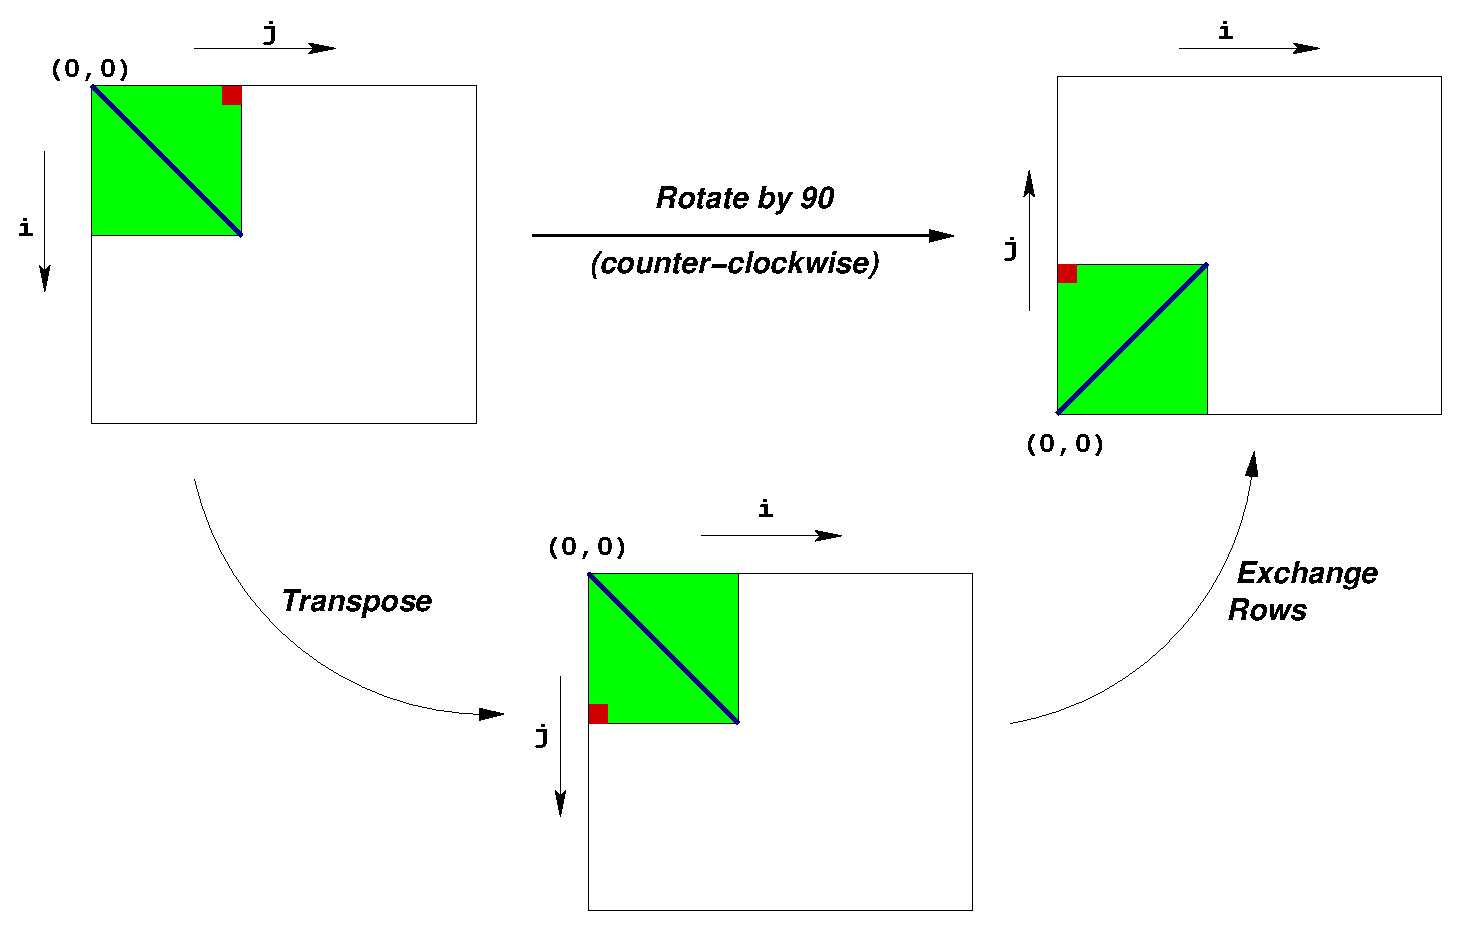
\epsfig{file=rotate.eps, width=4.5in}}
\caption{Rotation of an image by $90^\circ$ counterclockwise}
\label{fig:rotate}
\end{figure}
\begin{figure}[htbp]
\centerline{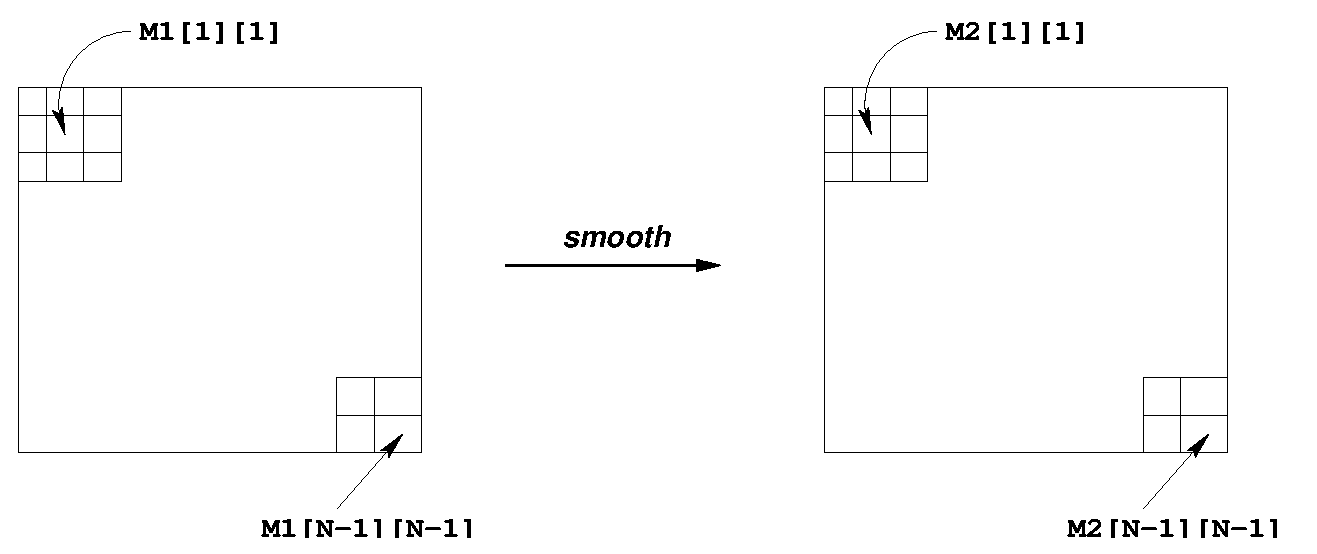
\epsfig{file=smooth.eps, width=4.5in}}
\caption{Smoothing an image}
\label{fig:smooth}
\end{figure}

\section{Logistics}
You should work alone on this assignment but may discuss it with
classmates as well as with the instructor. Final sumbissions should be made
via the handin script as assignment labperf.
Any clarifications and revisions to the assignment will be posted on
the course Web page.

\section{Hand Out Instructions}

\begin{quote}
The file perflab-handout.tar is available to copy from /home/comp235/ on
the linux server.
\end{quote}

Start by copying \texttt{perflab-handout.tar} to a protected directory
in which you plan to do your work.  Then give the command:
\verb@tar xvf perflab-handout.tar@.  This will cause a number of files
to be unpacked into the directory.  The only file you will be
modifying and handing in is {\tt kernels.c}.  The {\tt driver.c}
program is a driver program that allows you to evaluate the
performance of your solutions. Use the command \verb@make driver@ to
generate the driver code and run it with the command \verb@./driver@.

Looking at the file {\tt kernels.c} you'll notice a C structure {\tt
team} into which you should insert the requested identifying
information about the one or two individuals comprising your
programming team.  {\bf Do this right away so you don't forget.}


\section{Implementation Overview}
\label{sec:overview}
\subsection*{Data Structures}
The core data structure deals with image representation. A {\tt pixel} is
a struct as shown below:
\small{\begin{verbatim}
typedef struct {
   unsigned short red;   /* R value */
   unsigned short green; /* G value */
   unsigned short blue;  /* B value */
} pixel;
\end{verbatim}}
As can be seen, RGB values have 16-bit representations (``16-bit color''). An image {\tt I}
is represented
as a one-dimensional array of {\tt pixel}s, where the $(i,j)$th pixel
is {\tt I[RIDX(i,j,n)]}. Here {\tt n} is the dimension of the image
matrix, and {\tt RIDX} is a macro defined as follows:
\small{\begin{verbatim}
#define RIDX(i,j,n) ((i)*(n)+(j))
\end{verbatim}}
See the file {\tt defs.h} for this code.

\subsection*{Rotate}
The following C function computes the result of rotating
the source image {\tt src} by $90^\circ$ and stores the result in
destination image {\tt dst}. {\tt dim} is the dimension of the image.
\small{\begin{verbatim}
void naive_rotate(int dim, pixel *src, pixel *dst) {
  int i, j;

  for(i=0; i < dim; i++)
    for(j=0; j < dim; j++)
      dst[RIDX(dim-1-j,i,dim)] = src[RIDX(i,j,dim)];

  return;
}
\end{verbatim}}
The above code scans the rows of the source image matrix, copying to
the columns of the destination image matrix.
Your task is to rewrite this code to make it run as fast as
possible using techniques like code motion, loop unrolling
and blocking.

See the file {\tt kernels.c} for this code.

\subsection*{Smooth}
The smoothing function takes as input a source image {\tt src} and
returns the smoothed result in the destination image {\tt dst}.
Here is part of an implementation:
\small{\begin{verbatim}
void naive_smooth(int dim, pixel *src, pixel *dst) {
  int i, j;

  for(i=0; i < dim; i++)
    for(j=0; j < dim; j++)
      dst[RIDX(i,j,dim)] = avg(dim, i, j, src); /* Smooth the (i,j)th pixel */

  return;
}
\end{verbatim}}
The function {\tt avg} returns the average of all the pixels around
the {\tt (i,j)}th pixel. Your task is to optimize {\tt smooth} (and
{\tt avg}) to run
as fast as possible. ({\em Note:} The function {\tt avg} is a local
function and you can get rid of it altogether to implement {\tt
smooth} in some other way.)

This code (and an implementation of {\tt avg}) is in the file {\tt kernels.c}.

\subsection*{Performance measures}
Our main performance measure is {\em CPE} or {\em Cycles per Element}.
If a function takes $C$ cycles to run for an image of size $N \times
N$, the CPE value is $C/N^2$.
Table \ref{tbl:cpes} summarizes the performance of the naive
implementations shown above and compares it against an optimized
implementation. Performance is shown for
for 5 different values of $N$. All measurements were made on the
Pentium III Xeon Fish machines.

The ratios (speedups) of the optimized implementation over the naive
one will constitute a {\it score} of your implementation.
To summarize the overall effect over different values of $N$,
we will compute the {\em geometric mean} of the
results for  these 5 values. That is,
if the measured speedups for $N=\{32, 64, 128, 256, 512\}$ are
$R_{32}$, $R_{64}$, $R_{128}$, $ R_{256}$,  and $ R_{512}$
then we compute the overall performance as
\begin{eqnarray*}
R & = & \sqrt[5]{R_{32} \times R_{64} \times R_{128} \times R_{256}  \times R_{512}}
\end{eqnarray*}

\subsection*{Assumptions}
To make life easier, you can assume that $N$ is a multiple
of 32.  Your code must run correctly for all such values of $N$, but
we will measure its performance only for the 5 values shown in Table
\ref{tbl:cpes}.


\begin{table}
\begin{center}
\begin{tabular}{|ll|rrrrr|r|}
\hline
\multicolumn{2}{|r|}{Test case}&1&2&3&4&5&\\
\hline
\hline
Method & N & 64 & 128 & 256 & 512 & 1024 & Geom. Mean \\
\hline
Naive {\tt rotate} (CPE)
&   & 14.7 &  40.1 &  46.4 &  65.9 &  94.5 & \\
\hline
Optimized {\tt rotate} (CPE)
&   & 8.0  & 8.6 &  14.8 &  22.1 &  25.3 & \\
\hline
Speedup (naive/opt)
&   &  1.8 &   4.7  & 3.1  &  3.0  &  3.7  &  3.1   \\
\hline
\hline
Method & N & 32 & 64 & 128 & 256 & 512 & Geom. Mean \\
\hline
Naive {\tt smooth} (CPE)
& & 695 & 698 & 702 & 717 & 722 & \\
\hline
Optimized {\tt smooth} (CPE)
& & 41.5 & 41.6 & 41.2 & 53.5 & 56.4 & \\
\hline
Speedup (naive/opt)
& & 16.8 &  16.8 & 17.0 & 13.4 & 12.8 & 15.2 \\
\hline
\end{tabular}
\end{center}
\caption{CPEs and Ratios for Optimized vs. Naive Implementations}
\label{tbl:cpes}
\end{table}

\section{Infrastructure}
We have provided support code to help you test the correctness of your
implementations and measure their performance. This section describes
how to use this infrastructure. The exact details of each part of the
assignment is described in the following section.

{\bf Note:} The only source file you will be modifying is {\tt
kernels.c}.

\subsection*{Versioning}
You will be writing many versions of the {\tt rotate} and {\tt smooth}
routines. To help you compare the performance of all the different
versions you've written, we provide a way of ``registering''
functions.

For example, the file {\tt kernels.c} that we have provided you
contains the following function:
\small{\begin{verbatim}
void register_rotate_functions() {
   add_rotate_function(&rotate, rotate_descr);
}
\end{verbatim}}
This function contains one or more calls to {\tt
add\_rotate\_function}. In the above example, \\
{\tt add\_rotate\_function}
registers the function {\tt rotate} along with a string {\tt
rotate\_descr} which is an ASCII description of what the function does.
See the file {\tt kernels.c} to see how to create the string
descriptions. This string can be at most 256 characters long.

A similar function for your smooth kernels
is provided in the file {\tt kernels.c}.

\subsection*{Driver}
The source code you will write will be linked with object code that we
supply into a {\tt driver} binary. To create this binary, you will
need to execute the command
\small{\begin{verbatim}
unix> make driver
\end{verbatim}}
You will need to re-make driver each time you change the code in
{\tt kernels.c}.
To test your implementations, you can then run the command:
\small{\begin{verbatim}
unix> ./driver
\end{verbatim}}
The {\tt driver} can be run in four different modes:
\begin{itemize}
\item {\em Default mode}, in which all versions of your implementation are run.
\item {\em Autograder mode}, in which only the {\tt rotate()} and
{\tt smooth()} functions are run. This is the mode we will run in when
we use the driver to grade your handin.
\item {\em File mode}, in which only versions that are mentioned in
an input file are run.
\item {\em Dump mode}, in which a one-line description of each version is
dumped to a text file. You can then edit this text file to keep only
those versions that you'd like to test using the {\it file mode}.
You can specify whether to quit after dumping the file
or if your implementations are to be run.
\end{itemize}

If run without any arguments, {\tt driver} will run all of your
versions ({\em default mode}).
Other modes and options can be specified by command-line arguments to {\tt
driver}, as listed below:
\begin{description}
\item {\tt -g} : Run only {\tt rotate()} and {\tt smooth()} functions
({\em autograder mode}).
\item {\tt -f <funcfile>} :
Execute only those versions specified in \texttt{<funcfile>} ({\it file mode}).
\item {\tt -d <dumpfile>} : Dump the names of all versions to a dump file
called \texttt{<dumpfile>}, {\it one line} to a version ({\it dump mode}).
\item {\tt -q} : Quit after dumping version names to a dump file. To be
used in tandem with {\tt -d}. For example, to quit immediately after
printing the dump file, type \texttt{./driver -qd dumpfile}.
\item {\tt -h} : Print the command line usage.
\end{description}

\subsection*{Team Information}
{\bf Important:} Before you start, you should fill in the struct in
{\tt kernels.c} with information about you (name and email addresses).
This information is just like the one for the Data Lab.

\section{Assignment Details}

\subsection*{Optimizing Rotate (50 points)}
In this part, you will optimize {\tt rotate} to achieve as low a CPE
as possible.  You should compile {\tt driver} and then run it with the
appropriate arguments to test your implementations.

For example, running driver with the supplied naive version (for
{\tt rotate}) generates the output shown below:
\small{\begin{verbatim}
unix> ./driver
Teamname: bovik
Member 1: Harry Q. Bovik
Email 1: bovik@nowhere.edu

Rotate: Version = naive_rotate: Naive baseline implementation:
Dim             64      128     256     512     1024    Mean
Your CPEs       14.6    40.9    46.8    63.5    90.9
Baseline CPEs   14.7    40.1    46.4    65.9    94.5
Speedup         1.0     1.0     1.0     1.0     1.0     1.0
\end{verbatim}}

\subsection*{Optimizing Smooth (50 points)}
In this part, you will optimize {\tt smooth} to achieve as low a CPE
as possible.

For example, running driver with the supplied naive version (for
{\tt smooth}) generates the output shown below:
\small{\begin{verbatim}
unix> ./driver

Smooth: Version = naive_smooth: Naive baseline implementation:
Dim             32      64      128     256     512     Mean
Your CPEs       695.8   698.5   703.8   720.3   722.7
Baseline CPEs   695.0   698.0   702.0   717.0   722.0
Speedup         1.0     1.0     1.0     1.0     1.0     1.0
\end{verbatim}}

{\bf Some advice.} Look at the assembly code generated for the
\texttt{rotate} and \texttt{smooth}. Focus on optimizing the inner
loop (the code that gets repeatedly executed in a loop) using the
optimization tricks covered in class.  The \texttt{smooth} is more
compute-intensive and less memory-sensitive than the \texttt{rotate}
function, so the optimizations are of somewhat different flavors.

\subsection*{Coding Rules}
You may write any code you want, as long as it satisfies the following:
\begin{itemize}
\item
It must be in ANSI C.  You may not use any embedded assembly language
statements.
\item
It must not interfere with the time measurement mechanism.  You will
also be penalized if your code prints any extraneous information.
\end{itemize}
You can only modify code in {\tt kernels.c}.  You
are allowed to define macros, additional global variables, and other
procedures in these files.

\subsection*{Evaluation}

Your solutions for {\tt rotate} and {\tt smooth} will each count
for 50\% of your grade. The score for each will be based on the following:
\begin{itemize}

\item Correctness: You will get NO CREDIT for buggy code that causes
the driver to complain! This includes code that correctly operates on
the test sizes, but incorrectly on image matrices of other sizes. As
mentioned earlier, you may assume that the image dimension is a
multiple of 32.

\item CPE: You will get full credit for your implementations of
\texttt{rotate} and \texttt{smooth} if they are correct and achieve
mean CPEs above thresholds $S_r$ and $S_s$
respectively.  You will get partial credit for a correct
implementation that does better than the supplied naive one.
\end{itemize}

%\begin{quote}
%\bf SITE-SPECIFIC: As the instructor, you will need to decide on your
%full credit threshholds $S_r$ and $S_s$ and your rules for partial
%credits. We typically use a linear scale, with about a 40\% minimum if
%students actually tried to solve the lab.
%\end{quote}

\section{Hand In Instructions}

When you have completed the lab, you will hand in one file,
\verb@kernels.c@, that contains your solution.  Here is how to hand in
your solution:

\begin{itemize}
\item Make sure you have included your identifying information in
the team struct in {\tt kernels.c}.

\item Make sure that the {\tt rotate()} and {\tt smooth()} functions
correspond to your fastest implementations, as these are the only
functions that will be tested when we use the driver to grade your assignment.

\item Remove any extraneous print statements.

\item Create a team name of the form:
\begin{itemize}
\item ``${\it ID}$'' where ${\it ID}$ is your Andrew ID, if you are
working alone, or
\item ``${\it ID}_1${\tt +}${\it ID}_2$'' where ${\it ID}_1$ is the
Andrew ID of the first team member and ${\it ID}_2$ is the Andrew ID
of the second team member.
\end{itemize}
This should be the same as the team name
you entered in the structure in {\tt kernels.c}.

\item To handin your {\tt kernels.c} file, type:
\small{\begin{verbatim}
handin comp235 labperf kernels.c
\end{verbatim}}

\item After the handin, if you discover a mistake and want to
submit a revised copy, then you may retract and resubmit your code
as described with \verb{handin -h}.

\end{itemize}

Good luck!

\end{document}
